\documentclass{article}

% Degenerate Baselines in Agentic Benchmarks
% Camera-ready: the "final" option prints the author block and the workshop
% footer, and drops the line numbers.
\usepackage[dblblindworkshop, final]{neurips_2026}
% Printed in the first-page footer as "... (NeurIPS 2026). Workshop: <title>."
\workshoptitle{Who Verifies the Agents? Toward Reliable Agent Development}

\usepackage[utf8]{inputenc} % allow utf-8 input
\usepackage[T1]{fontenc}    % use 8-bit T1 fonts
\usepackage{hyperref}       % hyperlinks
\usepackage{xurl}           % URL typesetting, breakable at any character
\usepackage{array}          % >{...} column modifiers
\usepackage{booktabs}       % professional-quality tables
\usepackage{amsfonts}       % blackboard math symbols
\usepackage{amsmath}        % align, display math
\usepackage{amsthm}         % theorem environments
\usepackage{nicefrac}       % compact symbols for 1/2, etc.
\usepackage{microtype}      % microtypography
\usepackage{xcolor}         % colors
\usepackage{graphicx}       % figures

\theoremstyle{plain}
\newtheorem{proposition}{Proposition}
\theoremstyle{definition}
\newtheorem{definition}{Definition}

\newcommand{\floorcheck}{\texttt{floorcheck}}
\newcommand{\CR}{\mathrm{CR}}

\title{Mind the Floor: Closed-Form Degenerate Baselines for Agentic Benchmarks}

\author{%
  Dingyan Shang\\
  Capital One\\
  \texttt{dingyan.shang@capitalone.com}
}


\begin{document}

\maketitle

\begin{abstract}
  Scores on agentic benchmarks are routinely read as evidence of agent capability, yet some benchmark--metric pairs give substantial credit to a \emph{degenerate policy}: one that never reads its input. For many common metrics this score floor has a closed form that needs only label statistics and no agent rollout. It is also rarely reported. In a purposive sample of $29$ benchmark releases, $26$ of them agentic or tool-use, one reports a numeric input-oblivious baseline, and it is a static question-answering benchmark. None computes one on its released split. First, a taxonomy of degenerate-policy floors gives closed forms for ten metric families and an \emph{immune} family (balanced accuracy, Cohen's $\kappa$, MCC, ROC-AUC) on which every input-oblivious policy provably scores at chance in expectation. The binary hard-label cases restate the Dutch Draw, and multi-class balanced accuracy and $\kappa$ restate the \emph{equitability} criterion of forecast verification; multi-class macro-F1 and MCC, the pass@$k$ water-filling floor and the pass@$k$/pass$^{k}$ contrast are new. Second, an audit of nine public benchmarks ($18$ pairs) leads with each pair's \emph{headroom}, the distance from its floor to the metric's maximum. Headroom needs no ceiling estimate and does not change when better models appear. The audit finds that the floor is a real reporting issue but is severe only in a few designs. The large floors an agent can reach without reading its input appear where a benchmark scores declining or handing off a task. On BFCL's abstention slices, per-slice accuracy makes the floor the metric's \emph{maximum}. On $\tau$-bench airline, a constant transfer-to-human call passes the $19$ of $50$ tasks that need no database write and no communicated output. Third, we propose a half-page floor-report checklist and release \floorcheck{}, an open-source calculator that computes floors from a label file.
\end{abstract}

\section{Introduction}
\label{sec:intro}

Benchmarks for interactive agents have multiplied quickly. Function-calling suites, multi-turn tool-use dialogues, web navigation, embodied household tasks, and software-engineering environments each come with their own task distributions and scoring rules. A single headline number (an accuracy, an F1, a success rate) is then circulated as evidence that one agent is more capable than another, or that a model has ``learned to act.''

This paper asks what a policy that never reads its input scores on these benchmarks. We call such policies \emph{degenerate}: they emit a constant action, a constant answer, or an input-independent random draw. When a degenerate policy earns a large fraction of the state-of-the-art score on a benchmark, the benchmark's headline number overstates capability, just as $90\%$ accuracy does on a classification task that is $90\%$ negative.

The question goes back to 1884, when J.\,P.\ Finley reported tornado forecasts above $95\%$ ``percentage of verifications.'' Within months it was observed that never forecasting a tornado scores $98.2\%$ \citep{murphy1996finley}. Forecast verification began with a degenerate policy beating a published system; on $\tau$-bench airline today, one takes most of a published system's score (\S\ref{sec:results}).

Two facts make this worth a systematic treatment. First, for many metric families the degenerate floor has a \emph{closed form} computable from label statistics alone: the majority-class rate for accuracy, $2\pi/(1+\pi)$ for all-positive binary F1, at most $1/K$ for $K$-class macro-F1, and the other rows of Table~\ref{tab:closedforms}. Computing it takes seconds and no GPU time, but it is rarely reported beside the headline score. We coded $29$ benchmark releases, $26$ of them agentic or tool-use (\S\ref{sec:census}). Exactly one states such a baseline, and it is a static question-answering benchmark; none computes or normalizes against one. Second, one family of metrics (balanced accuracy, Cohen's $\kappa$, MCC, ROC-AUC) is provably \emph{immune}: every input-oblivious policy scores at chance. A constant policy does so exactly on every realization, and any other does so in expectation, up to an $O(1/n)$ term for $\kappa$ and MCC. The fix is therefore cheap: report the floor, or switch to an immune metric.

We make three contributions:
\begin{enumerate}
  \item \textbf{A floor taxonomy with closed forms} (\S\ref{sec:taxonomy}). We formalize degenerate policies, derive the best degenerate score for each common metric family, grouped into bands by what the floor depends on, and prove that balanced accuracy, $\kappa$, MCC and ROC-AUC are immune at any class count. New here are the multi-class macro-F1 marginal-matching optimum, multi-class MCC, the pass@$k$ water-filling floor, and the pass@$k$/pass$^{k}$ contrast. The ROC-AUC row is standard, since $\mathrm{AUC} = \nicefrac{1}{2}$ for an uninformative scorer is the ROC diagonal. Two groups of results restate prior work. The binary closed forms and binary immunity are those of \citet{vandebijl2022dutchdraw}. Multi-class balanced accuracy and $\kappa$ instantiate the \emph{equitability} criterion of \citet{gandin1992equitable}. That criterion is defined over categorical scoring matrices, so it covers neither multi-class MCC nor ROC-AUC.
  \item \textbf{An empirical audit} (\S\ref{sec:setup}--\S\ref{sec:results}). We audit nine public benchmarks ($18$ pairs). We run degenerate policies on BFCL, $\tau$-bench and ALFWorld, compute analytic floors for MMLU-Pro, GPQA diamond, GSM8K, WebArena and GAIA, and take floors fixed by the metric's definition for BFCL's abstention slices (a floor of $1$) and SWE-bench Lite (at least $1/n$). We report each pair's \emph{headroom}, $1 - \mathrm{floor}$, first, because it depends on the benchmark alone. The capture ratio $\CR = \text{floor}/\text{SOTA}$ is a dated secondary column, since SOTA changes as models improve. The panel's positive control is SWE-bench Lite, where the empty patch scores zero. Most agentic pairs have small floors, and the large floors appear where a benchmark scores declining or handing off a task.
  \item \textbf{A reporting protocol and tool} (\S\ref{sec:protocol}). Based on the audit, we propose a half-page floor-report checklist and release \floorcheck{}, a pip-installable calculator that computes all closed-form floors from a benchmark's label file.\footnote{Code and data: \url{https://github.com/dyshang/mind-the-floor}.}
\end{enumerate}

Our claims cover only the audited panel. Within it, headroom ranges from $0$ to $1$ across widely used pairs, and it is cheap to report.

\section{Related work}
\label{sec:related}

\paragraph{Null models against LLM judges.}
\citet{zheng2024cheating} showed that a ``null model'' emitting a fixed, input-agnostic response achieves high win rates on LLM-judged leaderboards such as AlpacaEval 2.0 \citep{dubois2024length}. We study the complementary case of agentic \emph{task} benchmarks scored by programmatic metrics, where the floor comes from label statistics.

\paragraph{Metric floors for trace judgment.}
Concurrent work co-authored by the present author \citep{wang2026safety} applies the all-positive F1 floor to safety trace judgment and reaches the same prescription as \S\ref{sec:immune}. The closed form there is the $\beta = 1$ case of \citet{vandebijl2022dutchdraw}, and none of the four benchmarks it audits appears in our panel.

\paragraph{Optimal input-independent baselines.}
The closest antecedent is the Dutch Draw \citep{vandebijl2022dutchdraw,pries2023optimal}. It constructs the optimal \emph{input-independent} binary classifier and gives closed forms for some $20$ confusion-matrix quantities, and a companion paper proves its optimality among input-independent classifiers for any order-invariant measure. Our binary closed forms and the binary cases of Proposition~\ref{prop:immune} restate theirs, credited at the point of use. Their baseline predicts a fixed \emph{number} of positives and shuffles which items receive them. Its draws are therefore exchangeable but not independent, so it sits just outside Definition~\ref{def:degenerate}. The two classes agree on every binary hard-label row of Table~\ref{tab:closedforms}, and where they differ (Proposition~\ref{prop:immune}(b)), theirs is the stronger statement. What is new beyond binary hard labels is listed in \S\ref{sec:intro}. Work on consistent optimization of macro-averaged metrics \citep{schultheis2024macroatk} treats the \emph{feature-dependent} Bayes-optimal classifier. A floor needs the input-oblivious special case, which is the one we study.

\paragraph{Reference forecasts and skill scores.}
\label{sec:skillscore}
Forecast verification began by scoring forecasts against policies that ignore their input. A \emph{skill score} is $(S - S_{\mathrm{ref}})/(S_{\mathrm{perfect}} - S_{\mathrm{ref}})$ for a chosen \emph{reference forecast}, usually climatology, persistence or chance \citep{jolliffe2012verification}. Checklist item~5 below is this quantity with the degenerate floor as the reference. A score is \emph{equitable} when every constant and every random forecast receives the same expected score \citep{gandin1992equitable}. That paper states the criterion for $K$ categories from the start, and it is what we call immunity. The split of Proposition~\ref{prop:immune} into (a) and (b) reproduces the distinction between strict and asymptotic equitability \citep{peirce1884,heidke1926,hogan2010equitability}, and Appendix~\ref{app:immune} gives the identities. The normalization is the same. Forecast verification fixes the reference by convention, while ours is a \emph{supremum over a declared policy class} (Definition~\ref{def:floor}) and so is a property of the benchmark.

\paragraph{Majority baselines, and how often the floor is reported.}
\label{sec:census}
Reporting a majority-class or random baseline was standard practice in classical NLP evaluation, and standard tooling still offers it (scikit-learn's \texttt{DummyClassifier}; \citealp{pedregosa2011scikit}). Such baselines have repeatedly exposed benchmarks solvable without their inputs \citep{kaushik2018reading,poliak2018hypothesis,gururangan2018artifacts} and progress that trivial baselines erase \citep{ferraridacrema2019progress}. To check whether the practice carried over to agentic evaluation, we coded a purposive frame of $29$ benchmark releases on the four questions of Appendix~\ref{app:census}. Of those $29$, one reports a numeric input-oblivious baseline (GPQA's nominal $25\%$ chance rate; \citealp{rein2023gpqa}), four reason about what an input-oblivious policy could exploit without reporting its score \citep{wang2024mmlupro,zhou2024webarena,xie2024osworld,wang2024mint}, none computes a floor on its released split, and none normalizes a headline score against one. That one is a static question-answering release, so over the $26$ agentic frame members the count is zero. The clearest of the four is OSWorld, which rewards an agent for declaring a task infeasible and does not report the $8.1\%$ that a constant \texttt{FAIL} scores, two-thirds of the score of its best reported agent. We resolved ambiguous cases toward counting a paper as reporting. The frame is purposive, so it shows the practice is rare among widely used agent benchmarks and gives no rate over all of them.

\paragraph{Abstention-aware and chance-aware evaluation.}
Another line of work evaluates when models should \emph{not} act: benchmarks of unanswerable or underspecified queries \citep{kirichenko2025abstentionbench,madhusudhan2026mmaqa}, training for calibrated refusal \citep{zhai2026abstainr1,gul2026mash}, and a survey \citep{wen2024abstention}. These works address the failure mode we formalize, an always-abstaining policy that saturates a naively scored refusal metric, and they motivate our immune-metric prescription for detection slices (\S\ref{sec:immune}). Work on repeated games argues for explicit null baselines on similar grounds \citep{papadopoulos2026coordination}. Where trajectories are scored with stateful partial credit \citep{lu2024toolsandbox,hallinan2026opaquetools}, no closed form exists, and our protocol handles this case with executed floors.

\paragraph{Benchmark quality audits.}
A validity literature asks which claims a benchmark score supports \citep{raji2021everything,bowman2021fix}. BetterBench \citep{reuel2024betterbench} and related checklists \citep{kapoor2024agents} assess benchmark construction quality broadly: documentation, statistical rigor, contamination, reproducibility. Closest to us is the Agentic Benchmark Checklist (ABC; \citealp{zhu2025abc}), which catalogs task-setup and reward-design defects and reports that they can move measured performance by up to $100\%$ in relative terms. It states our $\tau$-bench finding qualitatively, as ``$\tau$-bench counts empty responses as successful,'' so we treat ours as a quantitative replication. We give the number ($19/50$ airline, $7/115$ retail) and reproduce it with an execution-free counting identity. Beyond that, this paper adds closed forms that make a floor computable without a rollout, the floor-equals-maximum inversion, the immune-metric prescription, and a tool that emits the report, where ABC is filled in by hand.

\section{A taxonomy of degenerate floors}
\label{sec:taxonomy}

\subsection{Setup}

\begin{definition}[Degenerate policy]
\label{def:degenerate}
Let a benchmark be a finite set of tasks $\{(x_i, y_i)\}_{i=1}^{n}$ with inputs $x_i$, references $y_i$, and a metric $M$ mapping predictions to a score. A policy is \emph{degenerate} (input-oblivious) if its output distribution is independent of $x_i$: it emits either a constant prediction $c$ or a draw from a fixed distribution $q$ over outputs, \emph{and, across items, its outputs are mutually independent}. Where a metric scores $k$ samples per task we take the policy to be \emph{stateless}: the draws are i.i.d.\ and cannot condition on the trial index. This is an assumption about the harness. It holds where $k$ completions are drawn independently and fails where a policy can see what it has already emitted. Appendix~\ref{app:derivations} quantifies the difference.
\end{definition}

Proposition~\ref{prop:immune}(b), the McDiarmid bound of Appendix~\ref{app:immune} and the ROC-AUC exchangeability step all use the independence clause. Relaxing it to exchangeability at a fixed marginal gives the Dutch Draw class, on which Proposition~\ref{prop:immune}(b) becomes exact. A policy that depends only on item \emph{position} is input-oblivious but not index-invariant, and we treat it as a separate, harness-dependent class where it matters.

\begin{definition}[Floor, headroom, and capture ratio]
\label{def:floor}
The \emph{floor} of a benchmark--metric pair is the supremum of the expected score over the set $\Pi_{\mathrm{deg}}$ of degenerate policies $\rho$,
$\mathrm{floor}(B, M) = \sup_{\rho \in \Pi_{\mathrm{deg}}} \mathbb{E}\,[M(\rho, B)]$.
The \emph{headroom} is $1 - \mathrm{floor}$, on metrics whose maximum is $1$. The \emph{floor capture ratio} is $\CR = \mathrm{floor}/\mathrm{SOTA}$, where SOTA is the best published score on the same split and metric.
\end{definition}

The estimand is the \emph{released split}. A floor is a property of the $n$ tasks a benchmark ships, so the intervals we give cover policy randomness only, and the supremum is attained on every exact row of Table~\ref{tab:closedforms}.

The supremum over constant policies is always available by exhaustive search over observed labels, and for the metrics below it has a closed form. The \emph{floor} is a diagnostic property of the benchmark, computed from label statistics by whoever holds them, with no policy deployed. Running a degenerate \emph{policy} needs no label access, and on some audited pairs the maximizing policy is label-free anyway (a uniform guess on GPQA, constant abstention on BFCL), so the floor does not presume test-set access.

\subsection{Closed forms}
\label{sec:closedforms}

Table~\ref{tab:closedforms} summarizes the floors, with derivations in Appendix~\ref{app:derivations}. There $K$ is the number of classes, $\pi$ the positive-class rate, $p_c$ the empirical frequency of label $c$, $\hat{p}$ the vector of these, and $p_{\mathrm{mode}} = \max_c p_c$.

\begin{table}[t]
  \caption{Degenerate floors by metric family, grouped into bands by \emph{what the floor depends on}. Immunity (Proposition~\ref{prop:immune}) is stronger than a known floor, because it makes the four starred floors \emph{unbeatable} in expectation. AUPRC's entry is a lower bound, since average precision exceeds the asymptotic $\pi$ at finite $n$. Macro-F1's entry is an upper bound, since the marginal-matching draw reaches $1/K$ only as the rarest class grows; the value needs no label file, but the policy that approaches it does. \floorcheck{} emits \texttt{bound: lower} and \texttt{upper} for these two, \texttt{expectation} for $\kappa$ and MCC, and \texttt{exact} elsewhere. The two pass@$k$ rows are two policies for one floor, which is the larger value.}
  \label{tab:closedforms}
  \centering
  \small
  % Rows tightened a touch (not a font step) to keep the body inside nine pages.
  \renewcommand{\arraystretch}{0.92}
  \setlength{\tabcolsep}{4.5pt}
  \begin{tabular}{llll}
    \toprule
    Metric & Best degenerate policy & Floor & Inputs needed \\
    \midrule
    \multicolumn{4}{l}{\emph{Band A: floor depends on the label distribution; compute and report it}} \\
    Accuracy (single-label micro-F1) & majority class & $\max_c p_c$ & label counts \\
    Binary F1 & all-positive & $2\pi/(1+\pi)$ & positive rate \\
    Precision & all-positive & $\pi$ & positive rate \\
    AUPRC & random ranking & $\ge \pi$ (lower bound) & positive rate \\
    MCQ accuracy & modal option (or position) & $\max_c p_c$ & option counts \\
    Exact match (numeric) & modal answer & $p_{\mathrm{mode}}$ & answer counts \\
    pass@$k$ (deterministic) & modal answer & $p_{\mathrm{mode}}$ (all $k$) & answer counts \\
    pass@$k$ (stochastic, from $q$) & optimized $q$ & $\tfrac{1}{n}\sum_i [1-(1-q(y_i))^{k}]$ & answer counts \\
    pass$^{k}$ (all $k$ trials pass) & modal answer & $p_{\mathrm{mode}}$, flat in $k$ & answer counts \\
    \midrule
    \multicolumn{4}{l}{\emph{Band B: floor is fixed by the metric; state it once, no label file needed}} \\
    Recall & all-positive & $1$ & --- \\
    Macro-F1 ($K$ classes) & marginal-matching $q = \hat{p}$ & $\le 1/K$ (upper bound) & class count \\
    Balanced accuracy$^\star$ ($K$ classes) & (any) & $1/K$ & class count \\
    Cohen's $\kappa^\star$ & (any) & $0$ & --- \\
    MCC$^\star$ & (any) & $0$ & --- \\
    ROC-AUC$^\star$ (binary) & (any) & $\nicefrac{1}{2}$ & --- \\
    \midrule
    \multicolumn{4}{l}{\emph{Band C: no closed form; measure it}} \\
    LLM-judged win rate & canned response & high \citep{zheng2024cheating} & --- \\
    Partial credit / step score & constant action seq. & measured & rollout \\
    \bottomrule
  \end{tabular}
  \\[2pt]
  {\footnotesize $^\star$Immune (Proposition~\ref{prop:immune}): \emph{every} input-oblivious policy scores at chance in expectation, not merely the best one, and a constant policy scores exactly at chance on every realization. A randomized policy's single run scatters around chance (balanced accuracy by $\pm 0.21$ at $16$ positives; Appendix~\ref{app:immune}), and for $\kappa$ and MCC the expectation itself carries the $O(1/n)$ term of Proposition~\ref{prop:immune}(b).}
\end{table}

Binary F1's floor is already $0.67$ at $\pi = 0.5$, so F1 on balanced detection slices is especially exposed to floor inflation. For macro-F1 the optimal input-oblivious policy is a randomized draw \emph{matching the label marginals}. Its score reaches $1/K$ whatever the imbalance, the same constant as balanced accuracy's floor, though at finite $n$ only as an upper bound (Appendix~\ref{app:macrof1}).

The metrics pass@$k$ and pass$^{k}$ behave in opposite ways. Under pass@$k$, a task counts as solved if \emph{at least one} of $k$ samples is correct. A constant answer gains nothing from extra samples, but a stochastic guesser drawing i.i.d.\ from $q$ has per-item success $1-(1-q(y_i))^k$, so the floor \emph{grows with} $k$, and pass rates at large $k$ on small answer spaces inherit a large floor. Under pass$^{k}$ (the reliability metric $\tau$-bench reports), a task counts only if \emph{all} $k$ trials succeed. Randomizing is then strictly harmful, the optimum is the modal answer, and the floor stays at $p_{\mathrm{mode}}$ for every $k$. Moving from pass@$k$ to pass$^{k}$ thus removes everything a degenerate policy gains from extra samples. Both metrics assume a discrete answer space. Reward-scored trajectories, as in $\tau$-bench, have no answer histogram, so such pairs fall in Band~C.

\subsection{The immune family}
\label{sec:immune}

\begin{proposition}[Immunity]
\label{prop:immune}
Let $\hat{y}$ (a hard prediction over $K \ge 2$ classes) or $\hat{s}$ (a real-valued score, binary case) be produced by an input-oblivious policy, and let the task labels $y$ be fixed, with at least one item of each class. Write $\mathrm{BA}$ (balanced accuracy, i.e.\ macro-averaged recall), $\kappa$, $\mathrm{MCC}$, $\mathrm{AUC}$ for the empirical values on the panel.

\emph{(a) Deterministic constant policies.} If $\hat{y}$ (resp.\ $\hat{s}$) is constant across items, then on \emph{every} realization, exactly: $\mathrm{BA} = 1/K$; $\kappa = 0$; $\mathrm{MCC} = 0$ (taking the conventional value $0$ where the denominator vanishes); $\mathrm{AUC} = \nicefrac{1}{2}$ (ties counted half, the Mann--Whitney convention).

\emph{(b) Randomized i.i.d.\ policies.} If outputs are drawn i.i.d.\ across items from a fixed distribution, then $\mathbb{E}[\mathrm{BA}] = 1/K$ and $\mathbb{E}[\mathrm{AUC}] = \nicefrac{1}{2}$ \emph{exactly}, because their denominators (the per-class counts $n_{c}$, resp.\ $n_{+}n_{-}$) are fixed by the labels, never by the policy. Cohen's $\kappa$ and MCC are ratios with policy-dependent denominators, so they equal $0$ in expectation only up to the $O(1/n)$ bias of a ratio estimator. Concentration is governed by the \emph{smallest per-class count} $n_{\min} = \min_c n_c$, not by $n$: balanced accuracy and ROC-AUC fluctuate at rate $n_{\min}^{-1/2}$, and $\kappa$'s bound carries a $1/(1-\hat{p}_e)$ factor, with $\hat{p}_e$ the realized chance agreement, that blows up under extreme imbalance. Appendix~\ref{app:immune} gives explicit bounds for all four.
\end{proposition}

The proof (Appendix~\ref{app:immune}) rests on the fact that input-obliviousness makes $\hat{y}$ independent of $y$. Each class's recall then equals the unconditional rate at which the policy emits that class (a macro-average of $1/K$), observed agreement equals chance agreement, the prediction--label covariance vanishes, and every positive--negative score pair is exchangeable. The binary case of (a) is the Dutch Draw's \citep{vandebijl2022dutchdraw}, whose randomized branch is a \emph{stronger} statement on a neighboring class. Multi-class $\mathrm{BA}$ and $\kappa$ instantiate the equitability criterion of \citet{gandin1992equitable}; \S\ref{sec:intro} says which parts are new. Part (a) shows that the floor is \emph{at least} chance; reporting needs this direction, since the floor is a supremum. Part (b) shows that no input-oblivious policy \emph{exceeds} chance in expectation, up to the $O(1/n)$ term. \citet{heidke1926} applied the same correction to forecasters and \citet{cohen1960kappa} to annotators, for the same reason. The immune family applies it to a policy that ignores its input, and the census (\S\ref{sec:census}) shows that agent benchmarks have largely stopped doing so.

Immunity is stronger than having a known floor. Macro-F1 and balanced accuracy carry the \emph{same} constant $1/K$, and neither needs a label to write it down. For macro-F1, $1/K$ bounds a supremum that the modal constant falls strictly short of (Appendix~\ref{app:macrof1}). Under an immune metric, every input-oblivious policy scores chance in expectation, with no $O(1/n)$ term for balanced accuracy and ROC-AUC. For \emph{reporting} the difference does not matter, since only the supremum bounds what a degenerate policy can claim. It matters for \emph{interpretation}. Under an immune metric an input-oblivious policy's \emph{expected} score is chance, so a single run above chance shows input-dependence only once it clears the run-to-run band below.

Our central prescription follows the bands. \emph{If the floor depends on the label distribution (Band~A), compute and report it. If it is a structural constant (Band~B), state it once and normalize against it. If there is no closed form (Band~C), measure it with trivial policies.} Immune metrics are the part of Band~B where no input-oblivious policy beats the constant in expectation, and we recommend them for detection-style slices at any class count.

An immune metric is least stable where the imbalance that motivated it is worst. At the $16$ positives of the pooled BFCL task below, balanced accuracy has a $\pm 0.21$ band. Report the per-class counts beside it, and prefer balanced accuracy or MCC over $\kappa$ where the marginals are extreme \citep{feinstein1990kappa}. With only $16$ positives, no rescoring can fix the \emph{slice}, and collecting more positives is the better fix.

\section{Audit setup}
\label{sec:setup}

\paragraph{Panel.}
We audit three groups (Table~\ref{tab:panel}), separated by how the floor is obtained: \emph{executed} through the benchmark's own harness, \emph{analytic} from its label file, \emph{structural} from the metric's definition alone. A structural floor does not depend on any harness or seed. The argument gives exactly $1$ for BFCL's abstention slices and at least $1/n$ for SWE-bench Lite, since a constant policy can emit one task's gold patch. The groups follow the bands of Table~\ref{tab:closedforms} per \emph{pair}, not per metric family. GAIA, for example, is scored by exact match, a Band~A family, so it is analytic however open-ended its answers look (Appendix~\ref{app:benchmarks}). Checklist item~1 guards against judging a pair by how its answer space looks.

\paragraph{Sampling frame.}
The panel is purposive. Candidates needed a public split or label file and either a metric in Table~\ref{tab:closedforms} or a harness we could run unmodified, and the candidate list, with drops and reasons, ships with the artifact. As a result, the frame over-represents benchmarks with public label files, a trait plausibly correlated with \emph{lower} floors. Four of the $18$ pairs (GPQA, MMLU-Pro, both GSM8K rows) are static question answering, kept because pass@$k$ and MCQ floors have no agentic analogue.

\paragraph{Protocol.}
For executed benchmarks we fix all seeds, log every policy parameter and release per-episode JSONL. We select degenerate policies \emph{on the same information a benchmark card exposes}, without tuning on test scores. Configuration details are in Appendix~\ref{app:benchmarks}.

\section{Results}
\label{sec:results}

We report headroom first and treat every ceiling as a dated secondary annotation. We print only ceilings tied to a verified same-split primary source. Rows we could not attribute show ``---''. Their floors are at most $0.042$, or the metric's maximum for BFCL irrelevance, so no conclusion depends on their ceilings. Each printed ceiling is current as of its board's last update (2024-10 to 2026-08), recorded in \texttt{results/sota.json}, with the judgment calls in Appendix~\ref{app:sota}. Figure~\ref{fig:capture} and Table~\ref{tab:results} show the same $18$ pairs ordered by headroom.

\begin{figure}[t]
  \centering
  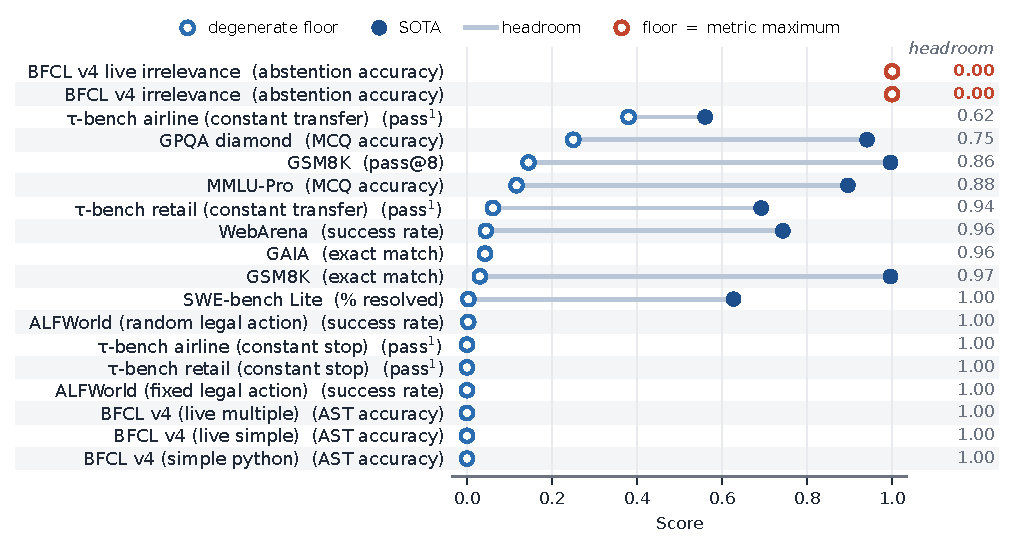
\includegraphics[width=\linewidth]{fig1_capture_ratio.pdf}
  \caption{Degenerate floor (open dot) vs.\ SOTA (filled dot) per audited pair, sorted by \emph{headroom} $1 - \mathrm{floor}$, the span a real agent can demonstrate. Pairs with floors near zero (bottom) offer nearly the full axis; on BFCL's abstention slices (top, warm) the floor is the metric's maximum and headroom is zero. Rows with no verified same-split ceiling are drawn floor-only, and their headroom is still defined. For executed pairs and WebArena the open dot is a lower bound.}
  \label{fig:capture}
\end{figure}


\paragraph{Headline.}
Headroom spans the full range. At zero headroom, BFCL's irrelevance slices score \emph{abstention} as accuracy over tasks where abstaining is correct by construction, so a policy that never calls a function is right on all $1{,}124$ of them. The floor is $1.0$, the metric's \emph{maximum}. Headroom is exactly zero, and the degenerate policy ties or beats every imperfect model without any leaderboard data, so no ceiling is needed. The cause is the slicing, since under per-slice accuracy \emph{any} single-label slice has floor $1.0$. The row is about a reporting practice, scoring such a slice on its own and folding it into a composite. BFCL v4 excludes the slice from its Live and Non-Live accuracy columns but keeps it inside \emph{Hallucination Measurement}, $10\%$ of the v4 composite \citep{bfcl2025v4scoring}. The inversion therefore reaches the composite at half to two-thirds of that category's weight and nowhere else (Appendix~\ref{app:benchmarks}), and it does not reorder the ranking.

Next, a constant \texttt{transfer\_to\_human\_agents} call passes $19$ of $\tau$-bench airline's $50$ test tasks (pass$^{1} = 0.38$, headroom $0.62$). Over the two ceilings attributable to the original harness, $\CR \in [0.68, 0.83]$, and we quote the best-documented one. The score is exact and replicates without execution (Appendix~\ref{app:benchmarks}). This row is the panel's Finley case, since a degenerate policy takes most of a real system's score on a \emph{mixed} task set. Deciding \emph{when} to refuse is a real capability, so the mechanism matters. The reward checks the final database state, and these $19$ tasks also require \emph{no communicated output}, so full credit is granted with no evidence that a refusal decision was made. The scoring rule cannot tell an agent that reasoned its way to a refusal from one that refuses unconditionally, and requiring a communicated justification would make the constant policy fail. Retail gives the same policy $7/115$, so the floor comes from the task mix rather than the harness.

\paragraph{The middle and the bottom of the panel.}
GPQA diamond's four-option format gives a uniform guesser $25\%$ (headroom $0.750$), the largest analytic floor. That $0.250$ is an expectation over shuffles, since GPQA leaves option order to the harness. On one realized shuffle the best constant \emph{position}, picked after the fact, scores $0.287$ on average ($95$th percentile $0.318$). A suite that fixes its shuffle should report that number (Appendix~\ref{app:benchmarks}). A stochastic guesser on GSM8K reaches $14.5\%$ at pass@8, $4.8\times$ its pass@1 floor. MMLU-Pro's modal option scores $11.7\%$, WebArena's unachievable tasks give a constant ``N/A'' $4.4\%$, and GAIA's answers concentrate on small integers, so the constant ``3'' scores $4.2\%$. At the bottom are the pairs on which the label-free policies we ran score almost nothing. Two mechanisms explain them: the verifier argument below, for SWE-bench Lite and BFCL's function-calling categories, and a combinatorial action space over multi-step success, for ALFWorld. The constant modal call fails BFCL's AST check on all $400/400$ simple entries ($397$ on the function name alone). ALFWorld's fixed policy succeeds on $0/134$ episodes and the random one on $8/2680$ over $20$ replicates (Wilson upper bound $0.006$, the panel's only sampled floor).

With the policies of Table~\ref{tab:panel}, nine of the $12$ agentic pairs score under $0.07$, and the three above it are the two abstention slices and $\tau$-bench airline. Constants built from the answer key score more on WebArena ($0.212$) and $\tau$-bench ($0.400$ airline, $0.096$ retail; Appendix~\ref{app:benchmarks}), which leaves seven of the $12$ under $0.07$, but no agent can run them without the labels. We group floors by mechanism. $\tau$-bench retail, for example, sits numerically with WebArena and GAIA, but we group it with airline because it shares the refusal channel, at a lower rate ($7/115$ against $19/50$). Verifiers over unbounded output spaces leave label-free policies almost nothing to score. The large label-free floors that remain come from a channel only interactive benchmarks have, in which declining to act is scored as if the agent had acted.

\begin{table}[t]
  \caption{Audit results, sorted by headroom. Src is how the floor was obtained (E executed, A analytic, S structural), per Table~\ref{tab:panel}. Headroom $= 1 - \mathrm{floor}$ needs no ceiling; $\CR$ is a dated secondary column, printed only where a verified same-split ceiling exists. LF marks floors that a \emph{label-free} policy attains, so an agent can reach them without the labels; MMLU-Pro is $(\approx)$ because its modal-option floor barely exceeds a uniform guesser's $0.111$. Three rows aggregate pairs sharing a floor and policy, so these $14$ rows cover $18$ pairs: four static question answering, two harness artifacts, and $12$ agentic pairs. Markers: $^{*}$lower bound, the best of the Table~\ref{tab:panel} policies (\S\ref{sec:results}), so headroom is an upper bound; $^\dagger$no verified same-split ceiling; $^\ddagger$floor $=$ the metric's maximum, so the inversion is structural; $^{\S}$ceiling contested, $\CR \in [0.68, 0.83]$; $^{\P}$frozen board, an upper bound. See Appendix~\ref{app:sota}.}
  \label{tab:results}
  \centering
  \small
  % Rows tightened a touch (not a font step) to keep the body inside nine pages.
  \renewcommand{\arraystretch}{0.92}
  \setlength{\tabcolsep}{3.6pt}
  \begin{tabular}{llrccrrr}
    \toprule
    Benchmark & Metric & Floor & Src & LF & Headroom & SOTA & $\CR$ \\
    \midrule
    BFCL v4 irrelevance & abstention accuracy & 1.000 & S & \checkmark & \textbf{0.000}$^\ddagger$ & ---$^\ddagger$ & ---$^\ddagger$ \\
    $\tau$-bench airline (constant transfer) & pass$^{1}$ & 0.380$^{*}$ & E & \checkmark & \textbf{0.620} & 0.560$^{\S}$ & 0.68$^{\S}$ \\
    GPQA diamond & accuracy & 0.250 & A & \checkmark & 0.750 & 0.941 & 0.27 \\
    GSM8K & pass@8 (stochastic) & 0.145 & A & & 0.855 & 0.996 & 0.15 \\
    MMLU-Pro & accuracy & 0.117 & A & ($\approx$) & 0.883 & 0.896 & 0.13 \\
    $\tau$-bench retail (constant transfer) & pass$^{1}$ & 0.061$^{*}$ & E & \checkmark & 0.939 & 0.692$^{\P}$ & 0.09$^{\P}$ \\
    WebArena & success rate & 0.044$^{*}$ & A & \checkmark & 0.956 & 0.743 & 0.06 \\
    GAIA & exact match & 0.042 & A & & 0.958 & ---$^\dagger$ & ---$^\dagger$ \\
    GSM8K & exact match & 0.030 & A & & 0.970 & 0.996 & 0.03 \\
    SWE-bench Lite & \% resolved & $\ge$0.003 & S & & $\le$0.997 & 0.627 & $\ge$0.005 \\
    ALFWorld (random legal action) & success rate & 0.003$^{*}$ & E & \checkmark & 0.997 & ---$^\dagger$ & ---$^\dagger$ \\
    ALFWorld (fixed legal action) & success rate & 0.000$^{*}$ & E & \checkmark & 1.000 & ---$^\dagger$ & ---$^\dagger$ \\
    $\tau$-bench (constant stop, both envs) & pass$^{1}$ & 0.000$^{*}$ & E & \checkmark & 1.000 & --- & --- \\
    BFCL v4 (simple / live) & AST accuracy & 0.000$^{*}$ & E & \checkmark & 1.000 & ---$^\dagger$ & ---$^\dagger$ \\
    \bottomrule
  \end{tabular}
\end{table}

\paragraph{Positive control.}
An empty patch scores exactly zero on SWE-bench Lite, whose verifier over an effectively unbounded output space demands constructive success. The floor is still not zero, because a constant policy that emits one task's gold patch resolves that task. It is therefore at least $1/n = 1/300$, with no bound from above. The same $1/n$ holds on BFCL's AST categories, whose checker accepts a fixed reference call, and on ALFWorld, where a constant plan replaying one game's expert solution solves it ($1/134$, above the random walk's $0.003$). The zeros in Table~\ref{tab:results} are what label-free policies score. GAIA looks like a positive control but is not one, because its scorer matches a \emph{released answer string} and those strings concentrate. BFCL's function-calling categories show the same thing on a smaller scale, since the AST check demands an exact function name and argument values. BFCL thus has both a near-zero metric and a floor-$1.0$ slice, and its composite does not show the difference.

\paragraph{Immune-metric reanalysis.}
The prescription of \S\ref{sec:immune} applies without changing a single task. We pool BFCL's v4 irrelevance slices ($1{,}124$ abstain-correct) with the live relevance slice ($16$ call-correct) into the one detection task they jointly describe. There the constant-abstain policy keeps raw accuracy $0.986$ but scores balanced accuracy $0.500$, $\kappa = 0$ and MCC $= 0$. These values are identities, exactly as Proposition~\ref{prop:immune}(a) requires (Appendix~\ref{app:immune}). Checking whether \emph{rankings} shift would need per-model per-slice predictions, which are not released, but the collapse of the floor to chance needs no model data.

\section{The floor-report protocol}
\label{sec:protocol}

We propose that benchmark releases include a short \emph{floor report}, and release \floorcheck{}, a pip-installable tool that produces one from a label file. The checklist (Figure~\ref{fig:checklist}) fits in half a page.

\begin{figure}[t]
\centering
\fbox{%
\begin{minipage}{0.92\linewidth}
\footnotesize
\textbf{Floor report checklist}
% Default list spacing put the box over half a page; the items are the content.
\begin{enumerate}
  \setlength{\itemsep}{1pt}\setlength{\parskip}{0pt}\setlength{\topsep}{2pt}
  \item \textbf{Band of the pair.} A if the floor depends on the label file, B if the metric and its declared class set fix it, C if neither. A metric absent from Table~\ref{tab:closedforms}, such as a success rate, is classified by this test.
  \item \textbf{Band A: compute it.} Report the floor from released label statistics ($\floorcheck$ \texttt{compute <labels>}) and say whether the maximizing policy needs them. Where the closed form is only asymptotic, as AUPRC's $\pi$ is, report it as a bound and say which way it errs.
  \item \textbf{Band B: state the constant.} Report it ($1/K$, $0$) and whether the metric is immune, i.e.\ whether \emph{every} input-oblivious policy sits at it or only the best one. No label file is needed.
  \item \textbf{Band C: measure it.} Run one constant-action, one random-action and one immediate-termination policy through the official harness, over $\ge 20$ replicates where stochastic; report the best as a lower bound over the policy class you name.
  \item \textbf{Headroom.} Report $1 - \mathrm{floor}$, which needs no ceiling and no re-dating, and give a score $s$ as $(s - \mathrm{floor})/(1 - \mathrm{floor})$ \emph{with an interval}: normalizing multiplies the standard error by $1/(1 - \mathrm{floor})$, so a high floor makes a gain less certain. If the floor equals the metric's maximum, the normalization is undefined and the metric should be replaced.
  \item \textbf{Capture ratio (dated).} If reporting $\CR = \mathrm{floor}/\mathrm{SOTA}$, date it, name the ceiling's source and split, and give a range when contested, because $\CR$ changes as models improve.
\end{enumerate}
\end{minipage}}
\caption{The floor-report checklist. \floorcheck{} emits items 1--3 and 5, and item~6 once given a ceiling and its source; item~4 needs a few rollouts of trivial policies.}
\label{fig:checklist}
\end{figure}

Item~5 matters most, because headroom stays fixed as models improve. Item~4 does not always need rollouts. Where a benchmark's reward is a function of its final state and its communicated output, and ground-truth action traces ship with the tasks, a Band~C floor is a counting identity over the released task files. This is how we reproduce the $\tau$-bench floor without the harness (Appendix~\ref{app:benchmarks}).

\paragraph{Who reports, and why.}
The checklist asks authors to publish a number that can make their own benchmark look weaker, and the evidence on reporting guidelines is mixed. In a randomized trial, a mandated hand-filled checklist did \emph{not} improve compliance \citep{hair2019iicarus}, while the NeurIPS reproducibility checklist raised code-submission rates \citep{pineau2021reproducibility}. We expect the difference to be who fills in the artifact, and here the tool emits items 1--3 and 5. A benchmarks track can also require a floor line, as it already requires a datasheet \citep{gebru2021datasheets}. Appendix~\ref{app:census} expands both arguments and discusses three cheap responses to a high floor.

Hidden test labels do not block the report. Band~B needs no label file, and Band~A needs at most the answer histogram, which the organizer already holds; only one scalar per metric leaves the server.

\section{Limitations and conclusion}
\label{sec:limitations}

\paragraph{Limitations.}
Our audit covers a purposive panel, and its frame over-represents benchmarks with public label files. Claims about agentic benchmarks rest on the $12$ agentic pairs, and the only large floor on a mixed task set, $\tau$-bench airline, comes from $50$ tasks. The reporting census is also purposive, and it codes reporting rather than awareness. Capture ratios are snapshots because SOTA changes, and the floors marked in Table~\ref{tab:results} are lower bounds. ALFWorld's two policies read the admissible-command list, so they sit just outside Definition~\ref{def:degenerate} (Appendix~\ref{app:benchmarks}). Showing general rank invalidity would need per-model per-slice predictions, which public leaderboards do not release. The exception is a floor equal to the metric's maximum, as on BFCL's abstention slices. It is a checkable sufficient condition for rank inversion, and checklist item~5 already asks for it. Elsewhere we claim only that a headline score remains usable for ranking, while its absolute scale is not meaningful without the floor.

\paragraph{Conclusion.}
Degenerate baselines are the cheapest experiment in agentic evaluation, and for most metrics the floor has a closed form. Every benchmark should report its floor or use an immune metric, and should report its headroom.

\bibliographystyle{plainnat}
\bibliography{references}

\appendix

\section{Derivations of closed-form floors}
\label{app:derivations}

Throughout, the benchmark has $n$ tasks with labels $y_1,\dots,y_n$; $p_c = \frac{1}{n}\lvert\{i : y_i = c\}\rvert$; in binary settings $\pi = p_{+}$.

\subsection{Accuracy}
A constant prediction $c$ scores $p_c$; the best constant is the majority class, giving $\max_c p_c$. A randomized input-oblivious policy with distribution $q$ scores $\sum_c q(c)\,p_c \le \max_c p_c$, so the deterministic majority policy is optimal among all degenerate policies.

\subsection{Binary F1, precision, recall}
This floor is the $\beta = 1$, all-positive case of the Dutch Draw closed forms \citep{vandebijl2022dutchdraw}, and is applied in the trace-judgment setting by \citet{wang2026safety}; we restate the derivation here because the taxonomy needs it, and claim no novelty for it. The all-positive policy has $\mathrm{TP} = n\pi$, $\mathrm{FP} = n(1-\pi)$, $\mathrm{FN} = 0$, hence precision $\pi$, recall $1$, and
\begin{equation}
  F_1 \;=\; \frac{2 \cdot \pi \cdot 1}{\pi + 1} \;=\; \frac{2\pi}{1+\pi}.
\end{equation}
For a randomized input-oblivious policy that predicts positive with probability $p$ independently of the label, $\mathbb{E}[\mathrm{TP}] = np\pi$, $\mathbb{E}[\mathrm{FP}] = np(1-\pi)$, $\mathbb{E}[\mathrm{FN}] = n(1-p)\pi$, giving plug-in precision $\pi$ and recall $p$, hence
$F_1(p) = 2\pi p/(\pi + p)$, which is strictly increasing in $p$; the maximum over $p \in [0,1]$ is attained at the deterministic all-positive policy $p = 1$, recovering $2\pi/(1+\pi)$. (This is the ratio-of-expectations plug-in; the expectation of the ratio on a finite panel differs at order $1/n$, which is negligible at benchmark sizes and does not change the maximizer.)

\subsection{Multi-class macro- and micro-F1}
\label{app:macrof1}
For single-label multi-class tasks, micro-F1 aggregates true/false positives over classes and reduces to accuracy, so its floor is $\max_c p_c$. For macro-F1, let an input-oblivious policy draw class $c$ with probability $q_c$. By independence, plug-in per-class precision is $p_c$ and recall is $q_c$, so
\begin{equation}
  \mathrm{macroF1}(q) \;=\; \frac{1}{K}\sum_{c} \frac{2\,p_c\,q_c}{p_c + q_c},
\end{equation}
a \emph{strictly} concave, separable objective over the simplex ($f_c'' = -4p_c^2/(p_c+q_c)^3 < 0$), so an interior stationary point is the global maximum. Stationarity requires $2p_c^2/(p_c+q_c)^2 = \lambda$ on the support; writing $q_c = \alpha p_c$, the constraint $\sum_c q_c = 1$ forces $\alpha = 1$. The optimum therefore \emph{matches the label marginals}, $q = \hat{p}$, giving $\mathrm{macroF1}(\hat p) = \frac{1}{K}\sum_c p_c = 1/K$. A declared class absent from the split contributes $F_1 = 0$ for every $q$, so the optimum places no mass there and matches marginals on the support, which returns the same $1/K$ over the declared set; \floorcheck{} implements that case explicitly. The best \emph{constant} policy (the modal class $m$) scores only $\frac{1}{K}\cdot\frac{2p_m}{1+p_m} < 1/K$: macro-F1 thus joins stochastic pass@$k$ as the entries of Table~\ref{tab:closedforms} whose degenerate optimum is randomized, not constant.

Unlike the binary case, the plug-in step here is not exact, and the direction of its error matters. The binary maximizer is deterministic, so its plug-in value is its realized value on every draw; the macro-F1 maximizer $q = \hat p$ is randomized, so $\mathbb{E}[\mathrm{macroF1}]$ and the ratio of expectations differ at finite $n$, at order $1/(n\,p_c)$, so the rarest class governs the gap. Over the \emph{exchangeable fixed-count} class of \citet{vandebijl2022dutchdraw}, $1/K$ is \emph{exact}: the denominator $n_c + \hat{n}_c$ is deterministic and $\mathbb{E}[\mathrm{TP}_c] = n_c\hat{n}_c/n$ by linearity. Over the i.i.d.\ class of Definition~\ref{def:degenerate} it is an \emph{upper} bound, approached as $n\min_c p_c \to \infty$, and the direction holds for every $q$, not only in simulation: given the number $m$ of items a policy labels $c$, those items are a uniformly random subset, so $\mathbb{E}[F_{1,c} \mid m] = 2mp_c/(np_c + m)$, which is concave in $m$, and Jensen's inequality bounds $\mathbb{E}[F_{1,c}]$ by the plug-in value $2p_cq_c/(p_c + q_c)$. Simulating five $(K, n)$ configurations (\texttt{scripts/check\_appendix\_numbers.py}) sizes the gap: $\mathbb{E}[\mathrm{macroF1}]$ falls short of $1/K$ by $0.0020$ at $K = 3$, $n = 60$ and by $0.0019$ at $K = 5$, $n = 200$, closing to within Monte Carlo error by $n = 1{,}140$. The gap errs in the direction a floor needs, the row is Band~B either way, and \floorcheck{} emits it as \texttt{bound: upper}. For multi-label micro-F1, the all-positive policy scores $2\bar{d}/(1+\bar{d})$ with $\bar{d}$ the mean label density, the direct analogue of the binary formula.

\subsection{AUPRC under random ranking}
A scorer that ranks items uniformly at random has expected precision $\pi$ at every fixed \emph{rank} cutoff: the items above it are an exchangeable sample, so the expected fraction of positives among them is $\pi$, the PR curve is flat at height $\pi$ in expectation, and the limiting AUPRC is $\pi$. This is the standard no-skill baseline for precision--recall curves \citep{saito2015prc}. Only the finite-panel correction below is ours.

That correction is one-sided and, unlike the exact entries beside it in Table~\ref{tab:closedforms}, not uniformly small. Average precision, the usual estimator, averages precision at the positions where positives \emph{land} rather than at fixed cutoffs, and conditioning on a positive occupying a position raises the precision there. The plug-in caveat of the binary F1 case thus has a definite sign here: $\mathbb{E}[\mathrm{AP}] > \pi$. On the pooled BFCL detection task of \S\ref{sec:results} ($n = 1{,}140$, $\pi = 16/1140 = 0.0140$), simulating uniformly random permutations ($40{,}000$ replicates, same script) gives $\mathbb{E}[\mathrm{AP}] = 0.0197$, a relative excess of $40\%$; at a milder $\pi = 0.10$ with $n = 1000$ the excess falls to $6\%$. The direction is conservative for a floor report, since the true degenerate score is higher than $\pi$ and never lower, but the excess is largest under the heavy imbalance that motivates detection metrics in the first place, so a benchmark reporting an AUPRC floor on a rare-positive slice should quote $\pi$ as a lower bound. Table~\ref{tab:closedforms} marks the row accordingly and \floorcheck{} carries the direction with the number, emitting \texttt{bound: lower} for AUPRC, \texttt{upper} for macro-F1 (Appendix~\ref{app:macrof1}), \texttt{expectation} for the two rows whose denominators the policy moves ($\kappa$ and MCC, per Proposition~\ref{prop:immune}(b)), and \texttt{exact} elsewhere.

\subsection{Multiple choice and exact match}
Identical to accuracy over the option (resp.\ answer-string) distribution: the best constant is the modal option/answer, with floor $p_{\mathrm{mode}}$. The constant \emph{position} policy is a separate, harness-dependent class (\S\ref{sec:taxonomy}): it scores the positional frequency, which exceeds $1/K$ for two distinct reasons. One is imperfect shuffling, the systematic case, and it is the same asymmetry that makes models themselves position-biased on multiple choice \citep{zheng2024selectors}. The other remains under perfect shuffling. On a realized shuffle, the best of $K$ positions is a maximum over $K$ correlated sample proportions, which is upward-biased at finite $n$ by the same finite-panel selection effect as the average-precision excess above. Appendix~\ref{app:benchmarks} quantifies it for GPQA diamond and says which of the two conventions the reported floor corresponds to.

\subsection{\texorpdfstring{pass@$k$}{pass@k}}
A deterministic constant answer $c$ succeeds on item $i$ iff $c = y_i$, independent of $k$: floor $p_{\mathrm{mode}}$. A stochastic policy drawing $k$ i.i.d.\ answers from $q$ succeeds on item $i$ with probability $1 - (1-q(y_i))^k$, giving
\begin{equation}
  \mathrm{floor}_k(q) \;=\; \frac{1}{n}\sum_{i=1}^{n}\Bigl(1 - \bigl(1 - q(y_i)\bigr)^{k}\Bigr),
\end{equation}
which is nondecreasing in $k$ and, for $k > 1$, is maximized by a $q$ that spreads mass over several frequent answers rather than the mode alone. The objective is concave in $q$ (each term is a composition of a concave function with an affine one), so the optimum is characterized by the KKT condition: writing $m_a$ for the count of answer $a$, every supported answer satisfies $m_a k (1-q_a)^{k-1} = \lambda$, i.e.\ $1 - q_a = (\lambda / k m_a)^{1/(k-1)}$, with $\lambda$ chosen so that $\sum_a q_a = 1$ and $q_a = 0$ for answers whose marginal value at zero, $m_a k$, falls below $\lambda$. Concavity makes this KKT point the global maximum, not merely a stationary one. This is a water-filling solution over the most frequent answers; \floorcheck{} solves it numerically. On GSM8K it lifts the floor from $3.0\%$ (deterministic, any $k$) to $14.5\%$ at $k=8$, over a support of $18$ answers; the full answer histogram is released in \texttt{results/analytic\_floors.json} so the floor, its support size, and the coverage figure below are recomputable offline. We use the naive $1 - (1-q)^k$ form. Harnesses that draw $n \ge k$ samples use the unbiased combinatorial estimator of \citet{chen2021codex}, and for an i.i.d.\ input-oblivious policy the two agree in expectation, since the policy's per-item success probability is constant across draws.

This optimum depends on the statelessness clause of Definition~\ref{def:degenerate}, so we quantify the clause here. A policy that returned the same fixed list of $k$ \emph{distinct} answers on every task reads no input either, but conditions on the trial index; on GSM8K the $8$ most frequent answers cover $267$ of $1{,}319$ items, so it would score $20.2\%$ against the $14.5\%$ above. We exclude it because a sampling harness draws $k$ completions independently and does not tell the model which draw it is on. The gap still shows that a floor depends on the benchmark, the metric \emph{and} the harness's sampling protocol. Under pass$^{k}$ nothing similar happens, because $k$ distinct answers cannot all match one reference. The modal-answer optimum of Appendix~\ref{app:passhatk} still holds in the wider class, and the contrast of \S\ref{sec:closedforms} only widens under it.

\subsection{\texorpdfstring{pass$^{k}$}{pass\^{}k}}
\label{app:passhatk}
The reliability metric pass$^{k}$ credits item $i$ only if \emph{all} $k$ independent trials succeed. A stochastic policy drawing i.i.d.\ from $q$ succeeds on item $i$ with probability $q(y_i)^k$, giving $\frac{1}{n}\sum_i q(y_i)^k$, which for $k \ge 1$ is maximized by placing all mass on a single answer (the objective is convex in $q$, so its maximum over the simplex is at a vertex) and hence by the modal answer, giving $p_{\mathrm{mode}}$. Randomization is strictly harmful for $k > 1$: any $q$ splitting mass across two or more answers scores strictly below $p_{\mathrm{mode}}$. The floor is thus $p_{\mathrm{mode}}$ for every $k$, flat where the pass@$k$ floor grows. Both metrics sit in Band~A because $p_{\mathrm{mode}}$ still depends on the answer histogram, but pass$^{k}$ denies a degenerate policy any benefit from extra samples.

\section{Immunity proofs}
\label{app:immune}

Let $\hat{y}$ be generated by an input-oblivious policy, so $\hat{y} \perp y$. For binary hard labels the balanced-accuracy, $\kappa$ and MCC arguments below are those of \citet{vandebijl2022dutchdraw}, restated here so the taxonomy is self-contained; the multi-class balanced-accuracy and $\kappa$ statements instantiate the equitability criterion of \citet{gandin1992equitable}, since those two are its Peirce and Heidke scores at $K$ categories. Equitability is defined over categorical scoring matrices, so neither multi-class MCC (whose $R_K$ form postdates that literature) nor ROC-AUC (not a categorical score at all) falls under it. ROC-AUC's $\nicefrac{1}{2}$ for an uninformative scorer is the ROC diagonal and standard elsewhere, so for ROC-AUC we add only its place in the taxonomy; \S\ref{sec:intro} lists which results are new.

\paragraph{The identities behind that attribution.}
Balanced accuracy is an affine rescaling of the Peirce skill score \citep{peirce1884}, $\mathrm{PSS} = \mathrm{TPR} - \mathrm{FPR} = 2\,\mathrm{BA} - 1$, so $\mathrm{PSS} = 0$ exactly when $\mathrm{BA} = \nicefrac{1}{2}$: our binary balanced-accuracy result is Peirce's, from 1884. Cohen's $\kappa$ is the Heidke skill score \citep{heidke1926}, $(\mathrm{PC} - \mathrm{PC}_{\mathrm{ref}})/(1 - \mathrm{PC}_{\mathrm{ref}})$ with the reference computed from the product of the marginals, published for weather forecasts $34$ years before \citet{cohen1960kappa} published it for annotators. An immune metric therefore has the item-5 normalization already built in, so Band~B and item~5 are two views of one idea. Finally, the split between our parts (a) and (b) is the known distinction between strict and asymptotic equitability: the Peirce score is strictly equitable while the widely used ``equitable threat score'' is only equitable in the large-sample limit \citep{hogan2010equitability}, exactly as our $\mathrm{BA}$ and $\mathrm{AUC}$ hold on every realization while $\kappa$ and MCC carry an $O(1/n)$ term. Forecast verification reached this distinction from a different failure mode, which supports the prescription.

\paragraph{Balanced accuracy.}
Balanced accuracy is macro-averaged recall, $\mathrm{BA} = \frac{1}{K}\sum_c \Pr(\hat{y}=c \mid y=c)$. Independence gives $\Pr(\hat{y}=c \mid y=c) = \Pr(\hat{y}=c) = q_c$, so $\mathrm{BA} = \frac{1}{K}\sum_c q_c = 1/K$. The per-class denominators $n_c$ are fixed by the labels and never by the policy, so this holds exactly in expectation and is not a ratio-estimator approximation. At $K = 2$ it reduces to the familiar $\mathrm{TPR} = \Pr(\hat{y}=+) = \mathrm{FPR}$ argument giving $\mathrm{BA} = \tfrac{1}{2}(\mathrm{TPR} + 1 - \mathrm{FPR}) = \nicefrac{1}{2}$.

\paragraph{Cohen's $\kappa$.}
Observed agreement $p_o = \sum_c \Pr(\hat{y}=c)\,p_c$ equals chance agreement $p_e$ computed from the marginals, because the joint factorizes; hence $\kappa = (p_o - p_e)/(1 - p_e) = 0$ in expectation. Nothing in this step depends on $K$, so it covers multi-class $\kappa$ unchanged, as does the covariance argument for MCC below. On a finite panel the empirical $\kappa$ fluctuates around $0$ at order $n^{-1/2}$; the statement is about the expectation, matching how the other floors are defined. The fluctuation is not symmetric under heavy imbalance. Simulating the pooled BFCL configuration below under the \emph{marginal-matching} policy $q = \pi$ ($n = 1{,}140$, $\pi = 16/1140$, $30{,}000$ replicates; \texttt{scripts/check\_appendix\_numbers.py}) gives a mean of $+1.3\times10^{-4}$ but a \emph{median} of $-0.013$, so a single run is more likely than not to report a small negative $\kappa$. The left shift comes from that policy rather than from $\kappa$ at this $n$: under the fair coin used for the bound below, the median is $0$. An organizer who runs the immune metric once should expect the shift, and read it as chance rather than as anti-correlation. When $p_e = 1$ (both marginals concentrated on one class) $\kappa$ is undefined and is conventionally set to $0$, consistent with the MCC convention below.

\paragraph{MCC.}
MCC is the Pearson correlation between prediction and label indicators; independence gives zero covariance, hence $\mathrm{MCC} = 0$ in expectation. For a constant prediction the denominator vanishes and MCC is conventionally set to $0$ \citep{chicco2020advantages}.

\paragraph{ROC-AUC.}
Empirical AUC is the Mann--Whitney statistic
$\frac{1}{n_+ n_-}\sum_{i: y_i = +}\sum_{j: y_j = -}\bigl(\mathbf{1}[s_i > s_j] + \tfrac12\mathbf{1}[s_i = s_j]\bigr)$.
A constant scorer ties every pair, giving exactly $\nicefrac{1}{2}$. For scores drawn i.i.d.\ from any fixed distribution, $(s_i, s_j)$ is exchangeable, so $\Pr(s_i > s_j) = \Pr(s_j > s_i)$ and every pair contributes $\nicefrac{1}{2}$ in expectation, hence $\mathbb{E}[\mathrm{AUC}] = \nicefrac{1}{2}$. (A ranking keyed to item \emph{position} is oblivious to input content but can exploit a dataset whose label order is not shuffled, in the same way as the constant-position MCQ policy of Appendix~\ref{app:derivations}; shuffling restores $\nicefrac{1}{2}$.)

\paragraph{The BFCL reanalysis, in full.}
BFCL's abstention behavior is naturally a binary detection problem, but the leaderboard scores the two classes as separate per-slice accuracies, so the abstain-only slices have a floor of $1.0$. Pooled into one detection task ($n = 1{,}140$, $16$ positives, counts read directly from \texttt{BFCL\_v4\_\{irrelevance, live\_irrelevance, live\_relevance\}.json}), a constant-abstain policy has $\mathrm{TPR} = 0$ and $\mathrm{TNR} = 1$ whatever the class ratio, so its balanced accuracy of $0.500$ is an identity, not a measurement: only the raw accuracy $0.986$ depends on the pool composition. Rescoring also makes the residual design problem visible in the same step, since the $70{:}1$ imbalance is what gives balanced accuracy the $\pm 0.21$ band computed above.

\paragraph{Finite-sample behavior.}
For \emph{deterministic constant} predictions the empirical values are exact, not asymptotic: $\widehat{\mathrm{BA}} = \nicefrac{1}{2}$, $\hat{\kappa} = 0$, $\widehat{\mathrm{MCC}} = 0$ (by the constant-prediction convention), and $\widehat{\mathrm{AUC}} = \nicefrac{1}{2}$ on every realization. For \emph{randomized} i.i.d.\ policies the statements hold in expectation with $n^{-1/2}$ fluctuations that can be made explicit. Let $\hat{N} = \hat{p}_o - \hat{p}_e$ be the numerator of $\hat{\kappa}$; $\mathbb{E}[\hat{N}] = 0$ exactly, and changing one prediction moves $\hat{N}$ by at most $2/n$, so McDiarmid's inequality gives, with probability at least $1-\delta$,
\begin{equation}
  |\hat{\kappa}| \;=\; \frac{|\hat{N}|}{1 - \hat{p}_e} \;\le\; \frac{1}{1 - \hat{p}_e}\sqrt{\frac{2\ln(2/\delta)}{n}}.
\end{equation}
On the pooled BFCL detection task of \S\ref{sec:results} ($n = 1{,}140$), a fair-coin policy satisfies $|\hat{\kappa}| \le 0.161$ at $\delta = 0.05$ \emph{with $\hat{p}_e$ at its realized value} $\nicefrac{1}{2}$ (rounded up, as a bound must be). The conditioning matters, because $\hat{p}_e$ is itself random, with a $97.5$th percentile of $0.528$ at this $n$, and a uniform statement needs a $\delta/2$ allowance for its fluctuation, which gives $0.193$. We quote both, since the first is the usable reporting recipe (an organizer observes $\hat{p}_e$ after the run) and the second is the unconditional bound.

Three features of these bounds are themselves diagnostic. First, the $\kappa$ bound degrades as $\hat{p}_e \to 1$: $\kappa$ is unstable when both marginals concentrate on one class, the same extreme-imbalance regime the reanalysis of \S\ref{sec:results} flags and the one the inter-rater literature warns about on structural grounds, not only on sample-size grounds \citep{feinstein1990kappa}. Second, the balanced-accuracy analogue concentrates \emph{per class}: by Hoeffding at $\delta/K$ per class, $|\widehat{\mathrm{BA}} - 1/K| \le \frac{1}{K}\sum_{c} \sqrt{\ln(2K/\delta)/(2 n_c)}$, which at $K = 2$ is the $\frac{1}{2}\sum_{c}\sqrt{\ln(4/\delta)/(2n_c)}$ we use; the minority class controls the width, and with $n_+ = 16$ call-correct tasks the band is $\pm 0.21$. Third, ROC-AUC is a two-sample U-statistic, so Hoeffding's inequality for U-statistics gives $\Pr(|\widehat{\mathrm{AUC}} - \nicefrac{1}{2}| \ge t) \le 2\exp(-2\min(n_+, n_-)t^2)$: the rate is $n_{\min}^{-1/2}$, as it is for balanced accuracy, and not $n^{-1/2}$. MCC's numerator has expectation exactly $0$ under the i.i.d.\ class, so its entire $O(1/n)$ term comes from the denominator and is not uniform in the imbalance. Immunity fixes the floor but does not reduce this sampling variance. A benchmark that adopts $\kappa$ on a slice with $16$ positives should therefore expect run-to-run swings of that width, prefer balanced accuracy or MCC there, and report the class counts alongside whichever it picks.

\section{Per-benchmark audit details}
\label{app:benchmarks}

\begin{table}[t]
  \caption{Audit panel, grouped by how the floor is obtained. \emph{Executed} floors are measured through each benchmark's official harness with fixed seeds. \emph{Analytic} floors are computed from public label statistics or released task configurations. \emph{Structural} floors follow from the metric's definition alone, with no execution and no label file: BFCL's abstention slices are structurally $1.0$, and SWE-bench Lite, the panel's positive control, is at least $1/n$, since the empty patch scores zero but a constant gold patch resolves its own task. \textbf{Band} is the Table~\ref{tab:closedforms} band of the \emph{pair} (\S\ref{sec:setup}).}
  \label{tab:panel}
  \centering
  \small
  \setlength{\tabcolsep}{4pt}
  \begin{tabular}{llcc>{\raggedright\arraybackslash}p{3.1cm}}
    \toprule
    Benchmark & Metric & Group & Band & Degenerate policy \\
    \midrule
    BFCL \citep{patil2024bfcl} & AST / exec.\ accuracy & executed & C & constant most-frequent function with default arguments \\
    $\tau$-bench \citep{yao2024tau} & pass$^{k}$ / reward & executed & C & constant \texttt{transfer\_to\_human}; immediate termination \\
    ALFWorld \citep{shridhar2021alfworld} & success rate & executed & C & repeated fixed legal action; uniform random legal action \\
    \midrule
    MMLU-Pro \citep{wang2024mmlupro} & MCQ accuracy & analytic & A & constant modal option \\
    GPQA diamond \citep{rein2023gpqa} & MCQ accuracy & analytic & A & uniform guess over four shuffled options \\
    GSM8K \citep{cobbe2021gsm8k} & exact match & analytic & A & modal answer \\
    WebArena \citep{zhou2024webarena} & success rate & analytic & A & constant ``N/A'' answer (scores the unachievable-task fraction) \\
    GAIA \citep{mialon2023gaia} & exact match & analytic & A & constant modal answer (``3'', $7/165$) \\
    \midrule
    BFCL irrelevance slices & abstention accuracy & structural & B & constant no-call (floor $=1$; metric counts abstention correct on every entry) \\
    SWE-bench Lite \citep{jimenez2024swebench} & \% resolved & structural & B & empty patch scores $0$; one task's gold patch gives floor $\ge 1/n$ (positive control) \\
    \bottomrule
  \end{tabular}
\end{table}

\subsection{BFCL v4: AST categories (executed), abstention slices (structural)}
Data and checker from the official \texttt{gorilla} repository (\texttt{bfcl\_eval}, cloned 2026-08-05). Audited categories: \texttt{simple\_python} ($n{=}400$), \texttt{live\_simple} ($n{=}258$), \texttt{live\_multiple} ($n{=}1{,}053$), plus the abstention slices \texttt{irrelevance} ($n{=}240$) and \texttt{live\_irrelevance} ($n{=}884$). Constant policy: the category's most frequent function name (e.g., \texttt{cmd\_controller.execute}, $28/258$ of \texttt{live\_simple} schemas) with schema-default arguments; deterministic, seed recorded as $0$. Predictions are scored by the unmodified official AST checker (\texttt{ast\_checker}); the wrapper feeds already-decoded calls, bypassing only the model-output string decoding. Result: $0/400$, $0/258$, $0/1{,}053$ valid ($397/400$ simple failures are function-name mismatches; the $28$ name matches in \texttt{live\_simple} all fail on argument values). The abstention slices are scored structurally: the metric counts abstention as correct on every entry, so constant no-call scores $1.0$ by definition and no rollout is possible or needed. Per-entry results for the AST categories: \texttt{results/bfcl\_eval\_*.jsonl}.

Slice sizes are read directly from the released v4 data files, and the pooled detection task of \S\ref{sec:results} depends on them: \texttt{BFCL\_v4\_irrelevance.json} has $240$ entries, \texttt{BFCL\_v4\_live\_irrelevance.json} has $884$, and \texttt{BFCL\_v4\_live\_relevance.json} has $16$. These differ from v3, where the corresponding live counts are $882$ and $18$: the live split holds $900$ relevance-detection entries in both versions, with two reclassified from call-correct to abstain-correct between them. The v4 numbers are the ones our floor uses; the v3 comparison is included so the counts can be checked against either release.

The same counts bound how far the inversion of \S\ref{sec:results} propagates. Constant abstention scores $1$ on both irrelevance slices and $0$ on live relevance, so within the $10\%$ \emph{Hallucination Measurement} category it collects $6.7$ points if the three slices are averaged equally and $5.0$ under an irrelevance/relevance grouping, and nothing anywhere else in the composite. Which of the two applies is fixed by \texttt{bfcl\_eval}'s category scorer, not by the published scoring description. We did not run that scorer, so we report the bracket. Either way the policy takes a fraction of one category, so \S\ref{sec:results} claims the inversion only for the slice and its category. The structural statement, that the floor equals the metric's maximum on the slice, needs no aggregation rule at all.

\subsection{ALFWorld (executed)}
Official \texttt{alfworld} package (TextWorld engine, \texttt{AlfredTWEnv}), \texttt{eval\_out\_of\_distribution} split ($134$ games), horizon $50$ steps, seed $0$. Policies: \emph{fixed} (first admissible ``go to'' command, else first admissible command, every step) and \emph{random} (uniform over admissible commands each step). Per-episode results: \texttt{results/alfworld\_\{fixed,random\}.jsonl}. Success rates: fixed $0/134 = 0.000$; random $1/134 = 0.007$ (a single episode where the uniform random walk completed a pick-and-place task within the horizon). Per the estimand fixed in \S\ref{sec:taxonomy}, a floor is a property of this released split, so only policy randomness needs an interval: the \emph{fixed} policy is deterministic and we report $0/134$ exactly, with no interval, while \emph{random} is run for the $20$ replicates checklist item~4 asks of a stochastic policy, seeds $0$--$19$, giving $8/2680 = 0.003$ with a Wilson $95\%$ interval of $[0.0015, 0.0059]$. Wilson is conservative here rather than exact, because the $134$ games are fixed distinct tasks: per-episode successes are independent but not identically distributed, and the Poisson-binomial variance of their mean is at most the binomial variance at the same mean. The claim needs only the interval's upper end, and even at $0.0059$ the headroom stays above $0.99$. The replicates also show the risk of using one seed. Only $14$ of the $20$ score zero and the most any scores is $2/134$, so seed $0$ alone catches one success and would put the random walk at $1/134 = 0.0075$, $2.5\times$ the $20$-replicate value, with an upper end of $0.041$ that $20$ replicates tighten sevenfold. Per-seed counts are in \texttt{results/alfworld\_random\_meta.json} with the harness versions, which matter here: TextWorld's grammar evaluator relies on pre-PEP-667 \texttt{locals()} behavior, so ALFWorld runs under Python $\le 3.12$ and every episode raises under $3.13$. Both policies also read the environment's state-dependent admissible-command list, which puts them just outside Definition~\ref{def:degenerate}, in a class that contains it. Their scores are therefore not an upper bound on the floor of Definition~\ref{def:floor}, and that floor is higher. A constant action sequence that replays one game's expert plan solves that game in this deterministic environment, so the floor is at least $1/134 = 0.0075$ (\S\ref{sec:results}). The combinatorial action space explains why policies that have memorized no plan score almost nothing, but it does not bound the floor. The $\tau$-bench and BFCL executed floors carry no interval because they are not sampled at all: the policies are deterministic, and for $\tau$-bench the counting identity below reproduces the transfer policy's score exactly.

\subsection{\texorpdfstring{$\tau$-bench}{tau-bench} (executed)}
Official \texttt{tau-bench} package (sierra-research), test splits, user simulator \texttt{claude-haiku-4-5} via the \texttt{llm} user strategy, seed $0$. Policies: \emph{transfer} (single constant \texttt{transfer\_to\_human\_agents} call, then terminate) and \emph{stop} (single canned refusal response, then terminate). Airline ($n{=}50$, the full test split): transfer passes $19/50 = 0.38$; stop passes $0/50$. Retail ($n{=}115$, the full test split): transfer passes $7/115 = 0.061$; stop passes $0/115$. The transfer floor is exactly the fraction of tasks whose reward-checked final database state equals the initial state \emph{and} that require no communicated output; the user-simulator model cannot affect it, because $\tau$-bench's reward is a function of those two quantities and a never-acting, never-communicating policy fixes both regardless of what the simulator says. Per-episode results: \texttt{results/tau\_\{env\}\_\{policy\}.jsonl}.

The floor admits an execution-free replication. A task passes under any never-writing policy iff replaying its ground-truth write actions leaves the database hash unchanged \emph{and} the task requires no communicated outputs; counting that predicate directly over the released task files (\texttt{scripts/executed/tau\_static\_floor.py}) reproduces $19/50$ (airline) and $7/115$ (retail) with per-task agreement of $50/50$ and $115/115$ against the executed runs. The per-task predicates are released as \texttt{results/tau\_\{env\}\_static\_floor.jsonl}, so that agreement is recheckable offline without installing the harness; \texttt{results/tau\_static\_floor.json} records the generating version, and a hash of the task set, which moves if upstream edits it. The predicate continues past a ground-truth action that raises, which assumes that an errored action leaves the database unchanged. Checking that assumption against the executed runs would be circular, since that agreement is what the identity is meant to establish, so the script counts the raising actions directly. The count is \emph{zero} in both environments. No ground-truth replay in either task set raises, so the identity needs no assumption on these task sets, and the count is what to re-check if the sets change. Regenerating the predicates needs the harness installed, the one step of this artifact that is not offline, and doing so reproduced the released predicates byte for byte at unchanged task-set digests. The executed floor is thus a counting identity of the task set, which the user-simulator model, prompts, seeds and harness sampling cannot move. The \emph{stop} policy's measured $0/50$ and $0/115$ reflect that a lone canned response does not terminate a $\tau$-bench episode, and an episode that never terminates scores $0$ by harness convention. An input-oblivious variant that repeats the refusal until the simulated user ends the dialogue would be scored by the same counting identity as \emph{transfer}; the $0.000$ rows are floors of the one-shot variant specifically, and the transfer rows are the binding $\tau$-bench floors among the policies we ran. A constant built from the answer key does better. One message that lists every expected output of the test tasks, followed by the transfer, also passes the never-write tasks that require an output: $20/50$ (airline) and $11/115$ (retail), by the same reward rule. This constant is degenerate but needs the labels, so the transfer rows keep their LF mark.

\subsection{MMLU-Pro, GSM8K, GPQA (analytic)}
Label files via HF \texttt{datasets}: \texttt{TIGER-Lab/MMLU-Pro} test ($n{=}12{,}032$; modal option ``A'' at $11.66\%$ vs.\ $11.09\%$ uniform), \texttt{openai/gsm8k} main/test ($n{=}1{,}319$; modal final answer ``5'' at $3.03\%$; stochastic pass@8 floor $14.47\%$ by the water-filling guesser of Appendix~\ref{app:derivations}). GPQA (\texttt{Idavidrein/gpqa}, config \texttt{gpqa\_diamond}, released as the \texttt{train} split, $n{=}198$; gated, accessed with an approved account): the modal answer text occurs in only $2.5\%$ of items, far below $1/4$, so the binding degenerate policy is the uniform guess over the four shuffled options, floor $0.250$. We audit the diamond split because published SOTA figures are reported on it, which keeps floor and ceiling on the same split; the floor is $0.250$ on the main split too.

The $0.250$ is an expectation over shuffles, and the dataset itself fixes which convention that is: GPQA ships the correct answer and its three distractors in separate columns, so the option \emph{order} is produced by the evaluation harness, and a harness that reshuffles per run gives each position $1/4$ in expectation. On any one realized shuffle the best constant-\emph{position} policy instead scores $\max_j \hat{p}_j$, which is upward-biased at finite $n$. Simulating uniform shuffles at $n = 198$, $K = 4$ ($200{,}000$ replicates; \texttt{scripts/gpqa\_position\_floor.py}, results in \texttt{results/gpqa\_position\_floor.json}) gives $\mathbb{E}[\max_j \hat{p}_j] = 0.287$, median $0.283$, $95$th percentile $0.318$. We report $0.250$ because the excess is not exploitable ex ante under a reshuffling harness. Still, a single GPQA run can give a constant-position policy nearly $0.29$, and a suite that fixes its shuffle at release should report $\max(1/4, \max_j \hat{p}_j)$ on the shuffle it ships.

\subsection{WebArena and GAIA (analytic); SWE-bench Lite (structural)}
SWE-bench Lite's empty patch resolves nothing, but its floor is not a structural zero. A constant policy that emits one task's gold patch resolves that task, so the floor is at least $1/n = 1/300$, the bound Table~\ref{tab:results} prints; we have not bounded it from above. GAIA's floor is measured exactly. Its $165$ released validation answers (\texttt{2023/validation/metadata.parquet}, gated, accessed with an approved account) are counted by \texttt{scripts/analytic\_floors.py} under the three branches of GAIA's own scorer, which compares a numeric answer as a float, a comma-separated one elementwise, and the rest as normalized strings: the modal answer is ``3'' at $7/165 = 0.042$, and the next four are also single-digit integers, seven times the $1/n$ that one memorized answer guarantees. Raw string counting gives the same $0.042$, so the floor comes from the concentration of answers and not from normalization. The floor needs the answer file, so the row carries no LF mark, and it remains a row with no verified same-split ceiling. WebArena's floor is counted from the released \texttt{config\_files/test.raw.json} (retrieved 2026-08-05) by \texttt{scripts/analytic\_floors.py}: $36$ of $812$ tasks carry an ``N/A'' reference answer. The marker sits on the \texttt{fuzzy\_match} key, which WebArena's string evaluator special-cases: an ``N/A'' reference is checked by exact match against the prediction, without the LLM judge. A constant-``N/A'' policy is scored correct on exactly those $36$ and gets $4.43\%$, since nothing else in those tasks' evaluation has to pass: all $36$ declare \texttt{string\_match} as their only \texttt{eval\_type}, none carries a \texttt{program\_html} check, and \texttt{fuzzy\_match} is the only reference-answer key present. One task ($247$) carries a \texttt{reference\_url} field, but \texttt{url\_match} is absent from its \texttt{eval\_types}, so the harness never reads it. The per-task \texttt{eval\_types} are recorded in \texttt{results/webarena\_unachievable.json} so this is checkable without the upstream config. The mechanism, unachievable tasks scored by recognizing unachievability, is described by \citet{zhou2024webarena}. A constant built from the answer key does better. Of the $812$ tasks, $172$ are checked only by \texttt{must\_include} substring matches, so one answer that joins their $308$ distinct references passes all $172$ ($0.212$) under WebArena's string evaluator. This constant needs the labels. It shows that the floor of Definition~\ref{def:floor} is at least $0.212$, and the row prints the label-free $0.044$ with a lower-bound mark.

\subsection{SOTA reference scores}
\label{app:sota}
Capture ratios divide by a published SOTA on the same split and metric, which is a moving and occasionally ambiguous target. We record model, source, and retrieval date for every figure in \texttt{results/sota.json}, and note three judgment calls.

(i)~$\tau$-bench airline, the one row where the choice of ceiling moves a headline number. Two figures are attributable to the original v1 harness. The benchmark's own leaderboard is frozen at the late-2024 model set at $0.460$ (Claude 3.5 Sonnet), giving capture ratio $0.83$. Princeton's HAL leaderboard reports $0.560$ (o4-mini high) on the original TAU-bench Tool Calling scaffold, with few-shot results removed in December 2025 for test-set leakage \citep{hal2025taubench}; this is the best-documented same-harness figure, and we quote the resulting $0.68$. A third figure, $0.700$ for Claude Sonnet 4.5, appears on an aggregator page labeled TAU-bench Airline and would be the most conservative available ceiling. It fails a provenance check, and we exclude it. The score is reported alongside retail $0.862$ and \emph{telecom} $0.980$, and the telecom domain exists only in $\tau^2$-bench \citep{barres2025tau2}, which ports airline and retail into a dual-control environment; the same source records a prompt addendum to the airline agent policy. So it is a $\tau^2$-bench number under a $\tau$-bench label, which the exclusion rule stated at the end of this paragraph already forbids. In general, a row that reports airline, retail \emph{and} telecom together is a $\tau^2$-bench row. Excluding it moves our capture ratio up, from $[0.54, 0.83]$ to $[0.68, 0.83]$. Figures reported directly on $\tau^2$-bench (airline $0.765$) are excluded for the same reason, since it is a different benchmark. The retail row has a milder version of the problem. Its $0.692$ comes from the frozen board, so the retail capture ratio of $0.09$ is an upper bound that any newer same-split figure would lower. The retail comparison that \S\ref{sec:results} relies on is between the two \emph{floors} ($19/50$ against $7/115$), and no ceiling enters it.

(ii)~Rows with no verified same-split ceiling print ``---'' in place of an estimate. This covers GAIA (the official validation leaderboard is closed, so no maintained same-split ceiling exists), the three BFCL AST categories (per-category columns are not exposed by any leaderboard or aggregator we could reach), and both ALFWorld policies (the available figures come from agent papers, with no maintained board). Author estimates could fill these cells without changing any conclusion, since their floors are at most $0.042$, so we leave the cells empty and use no denominator we cannot source. Their headroom, the quantity we report first, is unaffected.

(iii)~BFCL irrelevance is the one row where we decline a ceiling on principle, although a figure exists. The floor equals the metric's maximum, so the inversion holds against any model that is not perfect on the slice with no leaderboard data at all. The only published irrelevance figure we could locate ($0.877$) is reported on \emph{v3} while our floor is measured on v4 files, so dividing by it would produce a cross-version ratio ($1.14$) that is weaker evidence than the structural statement alone. We print ``---''.

\section{The reporting census, and two notes on adoption}
\label{app:census}

This appendix holds the census behind \S\ref{sec:census}, which asks one question of each benchmark release (whether the paper tells a reader what an input-oblivious policy scores on it), followed by the two adoption arguments \S\ref{sec:protocol} states in brief.

\paragraph{Frame.} Purposive, $29$ releases: the nine benchmarks of our own panel, plus $20$ widely used agentic or tool-use benchmark releases from 2023--2026 (AgentBench, ToolLLM/ToolBench, API-Bank, WebShop, Mind2Web, WebVoyager, VisualWebArena, WorkArena, MINT, AppWorld, TravelPlanner, ScienceAgentBench, MLAgentBench, TheAgentCompany, ToolSandbox, $\tau^2$-bench, AgentDojo, WindowsAgentArena, OSWorld, AgentBoard). It is not a random sample, so we report no confidence interval on it, and we release the full list so others can check the frame. All $29$ are coded.

\paragraph{Coding.} An \emph{input-oblivious} baseline is a policy that ignores the task input entirely: uniform random guessing, always predicting the majority or modal class, empty output, no-op, always abstaining, or a constant action. A human baseline, a weaker model, a retrieval system, a rule-based system that reads the instruction, and an ablated model are all excluded. Each paper is coded on four questions: (a) does it report a numeric score for such a policy on its own benchmark; (b) where does that number appear (abstract, headline table, prose or appendix, design rationale only); (c) is it computed on the released split or quoted as a nominal constant such as $1/K$; (d) is any headline score normalized against it. Full texts were extracted automatically and coded against these questions, and every ``yes'' was then adjudicated by hand against the quoted evidence. Three automatic ``yes'' codings were overturned to ``no'' because the named baseline reads the input: WebArena's human baseline, TravelPlanner's greedy search over the query's constraints, and WebShop's rule baseline, which searches the instruction text. Automatic extraction failed on three papers ($\tau$-bench, OSWorld, AgentBoard), which were coded by hand from the arXiv PDFs.

\paragraph{Result.} Of $29$: (a) $1/29$; (b) $1/29$ in a headline table; (c) $0/29$ computed on the released split; (d) $0/29$ normalized. Four papers reason about what an input-oblivious policy could exploit, a chance rate or a channel scoring abstention as correct, without reporting what such a policy would score. Defining such a channel does not qualify on its own. WindowsAgentArena inherits OSWorld's infeasible-task reward but does not discuss what an always-\texttt{FAIL} policy scores, and is coded absent. MMLU-Pro motivates its $10$-option format by the lower probability of a correct guess. WebArena documents the unachievable-task channel whose floor we compute in \S\ref{sec:results} without reporting what a constant ``N/A'' policy would score on it. OSWorld is the clearest case in the census, and one we would have liked to audit. Its action space includes \texttt{FAIL} (``agent decides the task is infeasible''), its reward awards $1$ ``if the agent accurately predicts failure for an infeasible task,'' and $30$ of its $369$ tasks are infeasible. A constant \texttt{FAIL} therefore scores $8.1\%$ against a best reported agent of $12.24\%$, a capture ratio of $0.66$. The paper observes the mechanism twice, noting that agents ``tend to easily output \texttt{FAIL} and refuse to continue trying,'' which ``leads to some false positives in infeasible tasks,'' and does not report the number. We derive it from that paper's own stated reward rule and task counts, without the released config or an executed run, so it is recorded here and has no row in Table~\ref{tab:results}. The per-paper coding sheet, with the evidence quoted for each call and each adjudication recorded, is \texttt{results/reporting\_census.json}.

\paragraph{Verification, and why no $\kappa$.} Every one of the $29$ was coded a second time on question (a) from the arXiv full texts, blind to the first pass's codes; the two passes agree on all $29$, and the pass produced one correction: MINT reads a random-guess baseline into its filtering rule (``we filter out instances that a random guess baseline can do well''), so we recode it from absent to design rationale. The second coder was an AI assistant reading the released texts, not a second human, and both passes share the same automated extraction, so a baseline that extraction misses is missed twice. This makes it a verification pass, not an independent replication. We do \emph{not} report Cohen's $\kappa$ on it. The marginal here is one \emph{yes} in $29$, so $p_e$ sits within $10^{-3}$ of $1$ and $\kappa$ is exactly the statistic Appendix~\ref{app:immune} warns about, its bound carrying a $1/(1-\hat{p}_e)$ factor that blows up under extreme imbalance; on this table it is $0/0$ to three decimals. We report raw agreement, the correction and this reason, since by our own analysis $\kappa$ carries no information at this marginal. The sheet is \texttt{results/census\_verification.json}.

OSWorld's Table~6 prints \texttt{Infeasible} at $8.13\%$ in its \emph{\% of Total} column, the share of the dataset that is infeasible. That is the same number, from the same $30/369$, as the score a constant \texttt{FAIL} collects, so the paper prints the floor in its own results table as a dataset property without treating it as a score.

\paragraph{What it does and does not support.} It supports the claim of \S\ref{sec:intro} that a floor is rarely reported beside a headline score on widely used agent benchmarks. It does not support a rate over all agentic benchmarks. It also codes what papers \emph{report}, not what their authors knew; several of these designs are visibly floor-aware, and the census counts reporting for that reason.

\paragraph{Who reports, expanded.} Two features of the checklist address the incentive not to report an unfavorable floor. Band~B admits no discretion, since stating a metric-fixed constant is a citation rather than a disclosure; and withholding Band~A's one scalar does not keep it private, since any third party holding the split can compute a proxy. The evidence on mandates is mixed. The IICARus randomized trial found that requiring a checklist at submission did not improve compliance \citep{hair2019iicarus}, while the NeurIPS reproducibility checklist raised code-submission rates at this venue \citep{pineau2021reproducibility}. Clinical prediction made comparison against exactly the two degenerate policies, treat-all and treat-none, standard practice through decision curve analysis \citep{vickers2006decision}. On our reading, the successes differ from the failure in whether a human fills the artifact in. Items 1--3 and 5 here are emitted by \floorcheck{} from the label file, so the argument makes a checkable prediction: item~4, the only hand-run item, is the one that will lapse.

\paragraph{Three cheap responses.} Each cheap response to a high floor has a cost. \emph{Deleting the slice}: the cheapest reply to a floor of $1.0$ on BFCL irrelevance is to drop the slice, which would remove the field's only abstention signal on function calling, where our own remedy (immune rescoring, \S\ref{sec:results}) changes no task at all. \emph{Escaping into Band~C}: item~4 owes only a lower bound over three hand-chosen policies, which is cheaper to produce and less revealing than Band~A's exact scalar, so a band claim should be justified rather than asserted, and a pair is Band~C because no closed form exists for it, not because our tool lacks one. \emph{Choosing a generous ceiling}: SOTA sits in $\CR$'s denominator, so a benchmark author lowers a reported ratio by citing the highest defensible ceiling. Item~6's dating and sourcing reduce the third risk, and the first two are the reason item~5, which needs no ceiling at all, matters most.

\section{\floorcheck{} usage}
\label{app:floorcheck}

Install: \texttt{pip install -e floorcheck/} (code and data: \url{https://github.com/dyshang/mind-the-floor}). Every command below runs as written from the repository root against the two sample label files shipped in \texttt{floorcheck/examples/}. Worked examples:
\begin{verbatim}
# label-based floors (accuracy / MCQ / exact match), labels as
# a JSON array ["A","B",...] or counts object {"A": 120, ...}
floorcheck compute floorcheck/examples/labels.json \
    --metric mcq_accuracy --sota 0.896

# stochastic pass@k floor (water-filling guesser); grows with k
floorcheck compute floorcheck/examples/answers.json --metric pass@k --k 8

# pass^k floor (all k trials must pass); flat in k
floorcheck compute floorcheck/examples/answers.json --metric 'pass^k' --k 8

# macro-F1 floor (1/K via marginal matching). It is a Band B row, so the
# declared class count alone is enough and no label file is needed:
floorcheck compute --metric macro_f1 --num-classes 10

# passing labels too adds the observed class count and the best *constant*
# policy's score, which is strictly below 1/K. Keep --num-classes when the
# declared label set is larger than the classes present in this split, as
# it is for examples/labels.json: 10 options declared, 8 realized.
floorcheck compute floorcheck/examples/labels.json \
    --metric macro_f1 --num-classes 10

# immune metrics: balanced accuracy is 1/K, so it takes --num-classes too
floorcheck compute --metric balanced_accuracy --num-classes 10

# rate-based binary floors
floorcheck compute --metric binary_f1 --pi 0.35 --sota 0.7

# checklist item 5: headroom is always emitted; pass --score for the
# headroom-normalized (s - floor) / (1 - floor)
floorcheck compute floorcheck/examples/labels.json \
    --metric accuracy --score 0.82

# checklist item 6: a capture ratio is a dated claim about one ceiling, so
# give low:high where the ceiling is contested, as tau-bench airline's is
floorcheck compute --metric precision --pi 0.38 --sota 0.46:0.70 \
    --sota-source "frozen board / HAL / aggregator" --sota-as-of 2024-10

# everything applicable at once. A ceiling and a score belong to one metric,
# so report will not spread them across rows without --for-metric
floorcheck report floorcheck/examples/labels.json --num-classes 10 \
    --sota 0.82 --for-metric accuracy
\end{verbatim}
Every result carries \texttt{band}, \texttt{label\_free}, \texttt{headroom} and \texttt{bound} fields, which are checklist items 1, 2 and 5. \texttt{bound} is \texttt{exact} on every row whose floor is a finite-panel supremum, \texttt{lower} on AUPRC, whose $\pi$ is asymptotic and understated at finite $n$, \texttt{upper} on macro-F1, whose $1/K$ the i.i.d.\ draw only approaches, and \texttt{expectation} on $\kappa$ and MCC (Appendix~\ref{app:derivations}). Where the floor equals the metric's maximum, \texttt{normalized\_score} is emitted as \texttt{null} with a note that the metric should be replaced (item~5), and the tool does not raise on the division by zero.
Table~\ref{tab:results} and Figure~\ref{fig:capture} are regenerated by \texttt{scripts/analytic\_floors.py}, \texttt{scripts/executed/bfcl\_score.py}, \texttt{scripts/collect\_results.py}, and \texttt{scripts/make\_figure1.py}, in that order; those scripts have their own dependencies, listed in \texttt{requirements-repro.txt}, while \floorcheck{} itself has none. Invoke the tool as \texttt{floorcheck} instead of importing it from the repository root, where the source directory shadows the installed package. The $36$ unachievable WebArena task ids are recorded in \texttt{results/webarena\_unachievable.json} so the count is auditable without the upstream configs; \texttt{analytic\_floors.py} takes \texttt{--webarena-config} to recount from those configs and cross-check the two, and every entry records which of the two produced it. Every derived figure the paper quotes (the Wilson intervals, the concentration bounds, the pooled slice arithmetic, the floor-growth ratio, the $\tau$-bench counting identity and its per-task agreement, and both Monte Carlo estimates) is recomputed and checked against its printed value by \texttt{scripts/check\_appendix\_numbers.py}, which runs offline from the released \texttt{results/} files and exits non-zero on any mismatch. The label-aware constants of Appendix~\ref{app:benchmarks} are recounted by \texttt{scripts/label\_aware\_webarena.py} (from the upstream WebArena configuration) and \texttt{scripts/executed/tau\_label\_aware.py} (with the $\tau$-bench package), and the check reads their results offline like the rest. The BFCL slice sizes it checks against are recorded, with each source file's SHA-256, in \texttt{results/bfcl\_slice\_counts.json}.

\end{document}
